\section{Beispiel 3}

\subsection{Ermittelung der 3dB Grenzfrequenz}

F"ur die Ermittelung der 3dB Grenzfrequenz wurde eine AC-Analyse verwendet.
Anschlie"send wurde aus den Bodediagrammen mittels Cursors die 3dB Grenzfrequenz ermittelt.
Das Bodediagramm ist in Abbildung \ref{fig:bode} zu sehen.
Dabei ergaben sich in der Simulation f"ur die beiden Modelle der Operationsverst"arker folgende Grenzfrequenzen.
\begin{enumerate}
 \item \textbf{LM324:} $f_g = 1.215 MHz$
 \item \textbf{LM324/NS:} $f_g = 1.379 MHz$
\end{enumerate}


\begin{figure}[h!]
 \centering
 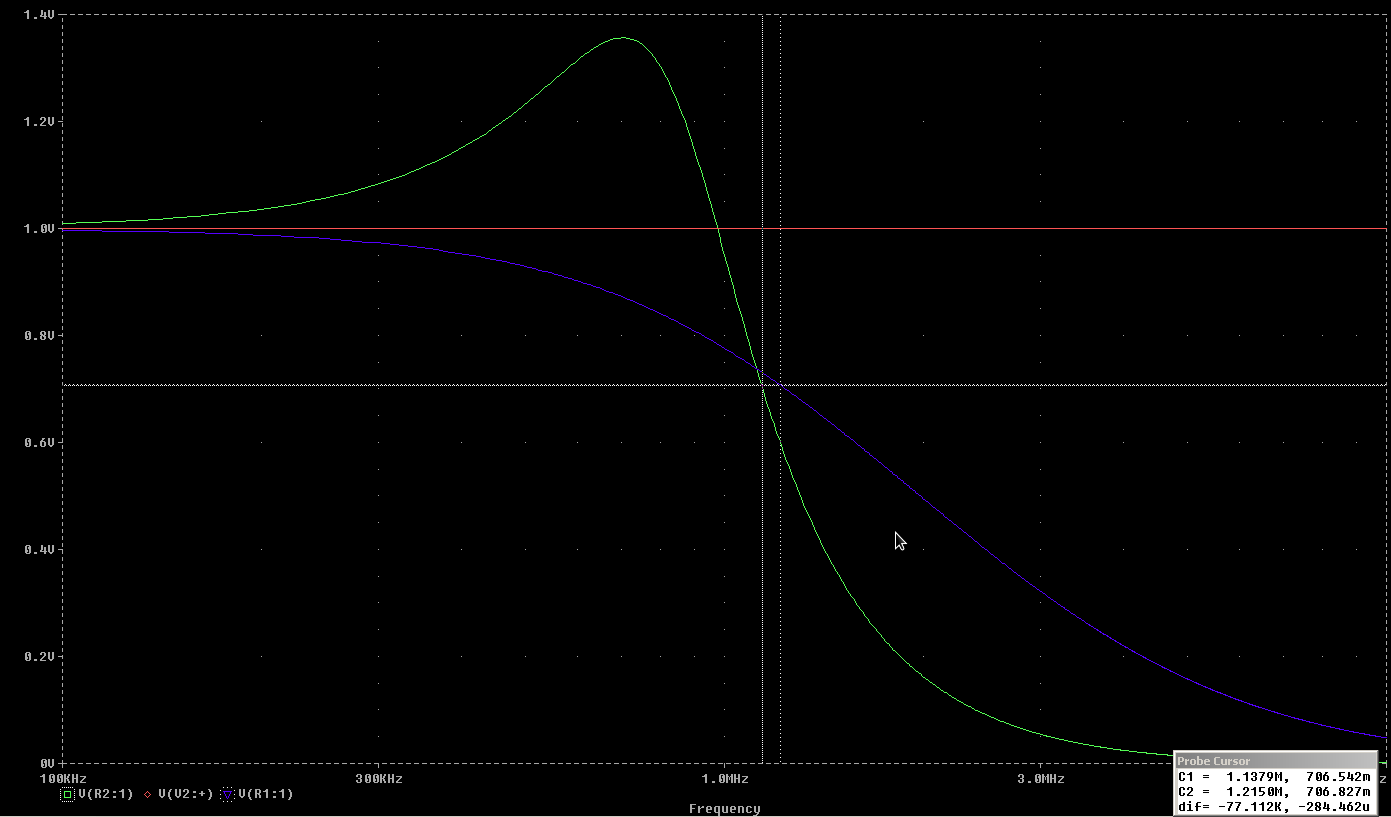
\includegraphics[width=16cm,keepaspectratio=true]{./fig/3_bode.png}
 % schalt2_ap.png: 1124x432 pixel, 72dpi, 39.65x15.24 cm, bb=0 0 1124 432
 \caption{Bode Diagramm der als Spannungsfolger beschaltenen OPVs. Der blaue Verlauf
 wurde mit dem PSPICE Modell LM324 ermittelt. Der gr"une Verlauf mithilfe des Models
 LM324/NS aus der Library nat\_semi.lib}
 \label{fig:bode}
\end{figure}

\subsection{Ermittelung der maximalen Frequenz mit THD < 1\%}

Die THD(Total Harmonic Distortion) kann mittels PSPICE ermittelt werden, indem man
bei der Transienten Analyse ``Enable Fourier'' aktiviert. Der von PSPICE ermittelte
Wert f"ur THD kann in der .out Datei abgelesen werden.
F"ur die Center Frequency wurde dabei die gleiche Frequenz wie f"ur die Eingangssinusschwingung verwendet.
Die Anzahl der Harmonischen wurde auf 50 eingestellt.

Nun wurde schwittweise die Frequenz verkleinert bzw. vergr"o"sert eine Frequenz ermittelt bei der
die THD kleiner 1\% betr"agt.

Dabei wurden folgende Frequenzen ermittelt:

\begin{enumerate}
 \item \textbf{LM324:} bei $f = 135 kHz$ betr"agt die THD 0,97\%.
 \item \textbf{LM324/NS:} bei $f = 133 kHz$ betr"agt die THD 0,97\%.
\end{enumerate}

\subsection{Zeitbereichsdarstellung bei den Grenzfrequenzen}
Die Zeitbereichsdarstellungen der Ausgangsspannungen der beiden Modelle bei den jeweiligen Grenzfrequenzen
sind in \ref{fig:3_lm324_fgzeitbereich} bzw. \ref{fig:3_lm324ns_fgzeitbereich} abgebildet.

Beim LM324 erkennt man, dass die Slew-Rate die Steigung der Ausgangsspannung begrenzt was zu
Verzerrungen f"uhrt.

Beim LM324/NS ist zus"atzlich eine niederfrequentere Schwinung "uberlagert, dies ist vermutlich
auf den Einschwingvorgang zur"uckzuf"uhren.

\begin{figure}[h!]
 \centering
 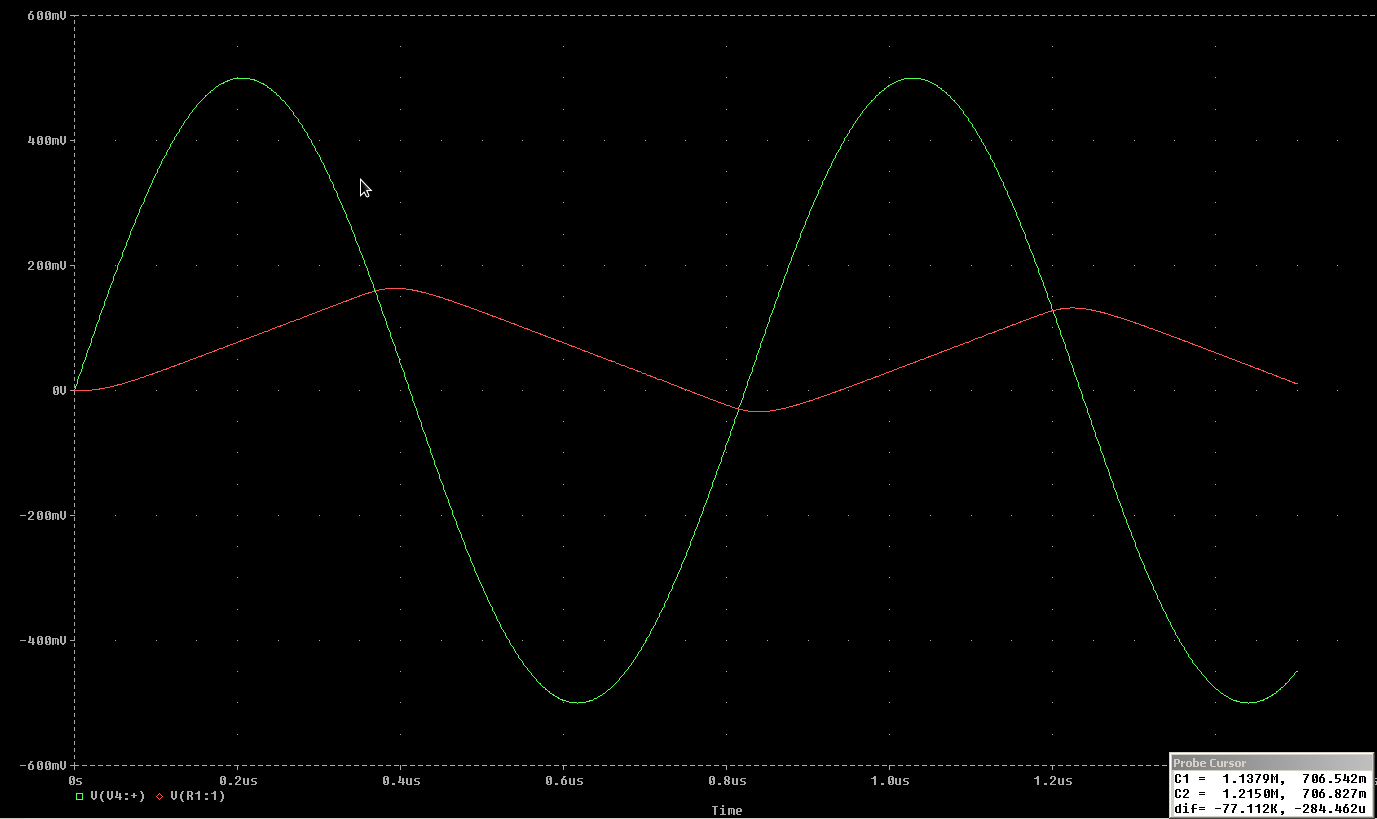
\includegraphics[width=16cm,keepaspectratio=true]{./fig/3_lm324_fgzeitbereich.png}
 % schalt2_ap.png: 1124x432 pixel, 72dpi, 39.65x15.24 cm, bb=0 0 1124 432
 \caption{Zeitbereichsdarstellung der Ausgangsspannung(rot) und Eingangsspannung(gr"un) bei der Grenzfrequenz des LM324.}
 \label{fig:3_lm324_fgzeitbereich}
\end{figure}

\begin{figure}[h!]
 \centering
 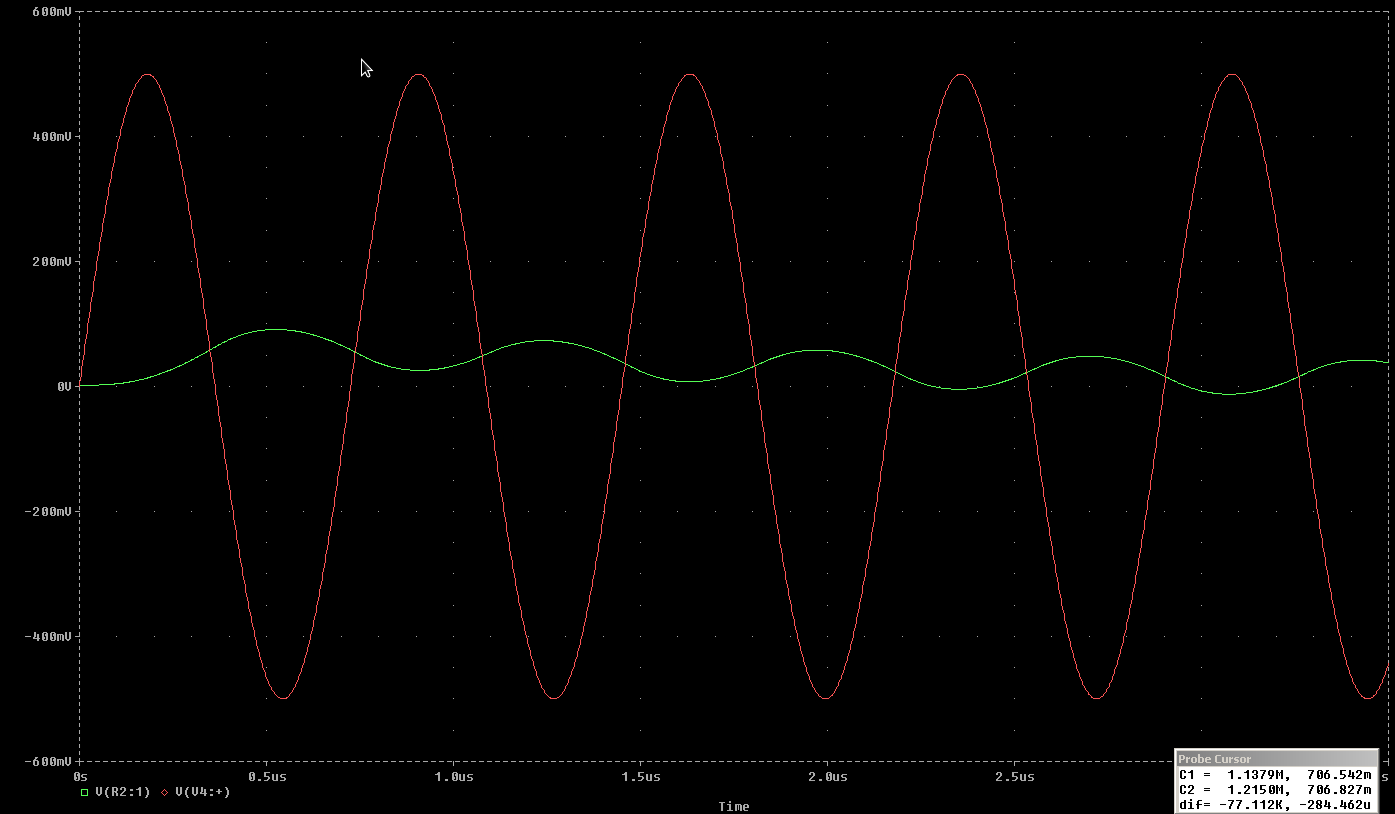
\includegraphics[width=16cm,keepaspectratio=true]{./fig/3_lm324ns_fgzeitbereich.png}
 % schalt2_ap.png: 1124x432 pixel, 72dpi, 39.65x15.24 cm, bb=0 0 1124 432
 \caption{Zeitbereichsdarstellung der Ausgangsspannung(rot) und Eingangsspannung(gr"un) bei der Grenzfrequenz des LM324/NS.}
 \label{fig:3_lm324ns_fgzeitbereich}
\end{figure}


\section{Beispiel 4}

Der Verlauf des ON-Widerstands des Transmissiongates ist in Abbildung \ref{fig:4_ron} abgebildet.
Man erkennt einen eine Unterschied des Wiederstands von ca. 250 Ohm zwischen den beiden Modellen.

\begin{figure}[h!]
 \centering
 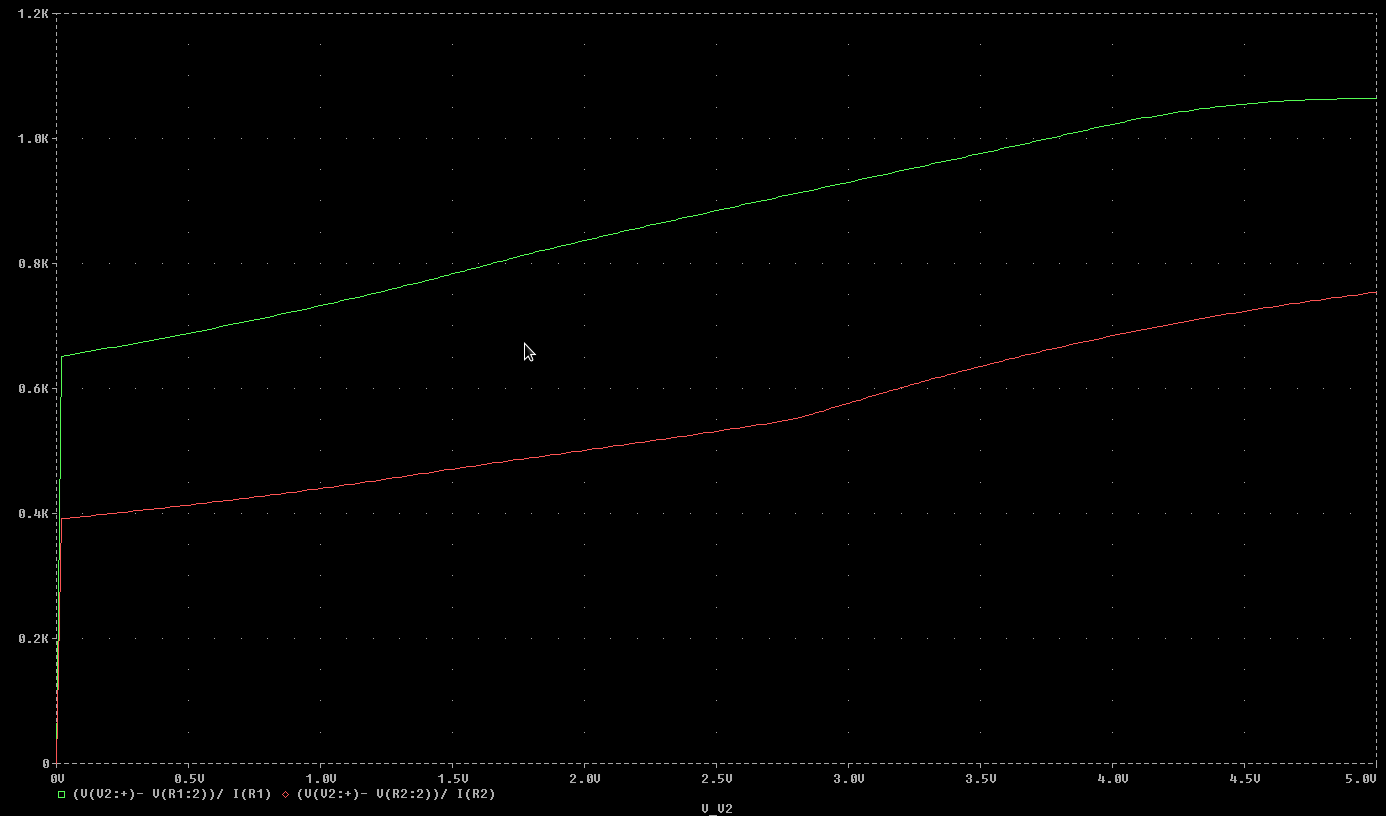
\includegraphics[width=16cm,keepaspectratio=true]{./fig/4_ron.png}
 % schalt2_ap.png: 1124x432 pixel, 72dpi, 39.65x15.24 cm, bb=0 0 1124 432
 \caption{$r_{on}$ (y-Achse) in Abh"angigkeit der geschalteten Spannung $V_{in}$ (x-Achse) der Modelle
 nmos,pmos(gr"un) bzw. nmos2,pmos2(rot)}
 \label{fig:4_ron}
\end{figure}
